% created on 27/04/2020
% @author : ebazan

\chapter{The uncertainty princple in the Gabor functions: This section needs to be reconstructed}

The uncertainty principle shows that the size, the shape and the shift of the window through which we make measurements affects the accuracy of what we compute. For example, let us consider a signal $f(t)$ with Fourier transform $F(\omega)$. Let us assume that we observe only a part of the signal through a window $w(t)$, with Fourier transform $W(\omega)$ centered at $t_0$

\begin{equation}\label{eq:uncertainty_principle2}
    h(t) = f(t)w(t-t_0)
\end{equation}


Due to the shifting property of the Fourier transform, the Fourier transform of the window is $e^{-j\omega t_0}W(\omega)$. Since the window multiplies the signal, the Fourier transform of the window is convolved with the Fourier transform of the signal. Therefore, the Fourier transform of what we observe is given by:

\begin{equation}\label{eq:short_time_fourier_transform}
    H(\omega) = \int_{-\infty}^{\infty}F(\omega - u)e^{-ju t_0}W(u) du
\end{equation}


In general $H(\omega)$ is different from $G(\omega)$ and depends on the locality of the window $t_0$.

The uncertainty principle shows that the size, the shape and the shift of the window through which we make measurements affects the accuracy of what we compute. For example, let us consider a signal $f(t)$ with Fourier transform $F(\omega)$. Let us assume that we observe only a part of the signal through a window $w(t)$, with Fourier transform $W(\omega)$ centered at $t_0$

\begin{equation}\label{eq:uncertainty_principle2}
    h(t) = f(t)w(t-t_0)
\end{equation}


Due to the shifting property of the Fourier transform, the Fourier transform of the window is $e^{-j\omega t_0}W(\omega)$. Since the window multiplies the signal, the Fourier transform of the window is convolved with the Fourier transform of the signal. Therefore, the Fourier transform of what we observe is given by:

\begin{equation}\label{eq:short_time_fourier_transform}
    H(\omega) = \int_{\infty}^{\infty}F(\omega - u)e^{-ju t_0}W(u) du
\end{equation}


In general $H(\omega)$ is different from $G(\omega)$ and depends on the locality of the window $t_0$.

To see this behavior, consider a signal $f(t)=A \sin \omega_{0} t$, where $A$ is a positive constant, and a window $w(t)$ defined by a Gaussian function. 

\begin{equation}\label{eq:1d_gaussian_function}
    w(t)=e^{-\frac{(t-t_0)^2}{2\sigma^2}}
\end{equation}
A Gaussian window is infinite in extent, so it is characterized by its locality $t_0$ and its standard deviation, which in this context is also called \textit{spread} and is denoted by $\sigma$. 

\begin{figure}
\centering
\subcaptionbox{}{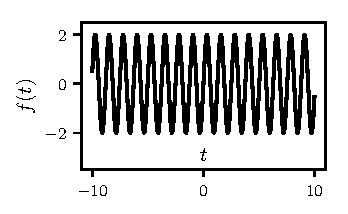
\includegraphics[width=0.325\textwidth]{sin_signal}\label{fig:sin_signal}}%
\subcaptionbox{}{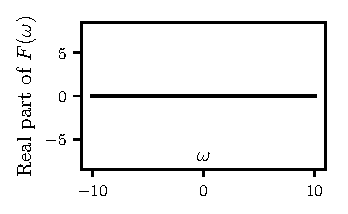
\includegraphics[width=0.325\textwidth]{real_sin_signal}}%\label{fig:sin_signal_real}
\subcaptionbox{}{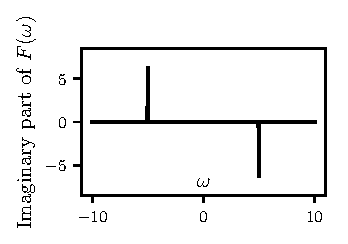
\includegraphics[width=0.325\textwidth]{imag_sin_signal}}\\%\label{fig:sin_signal_imag}
\hspace{0.33\textwidth}
\subcaptionbox{}{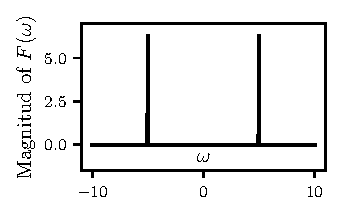
\includegraphics[width=0.325\textwidth]{mag_sin_signal}}%\label{fig:sin_signal_mag}
\subcaptionbox{}{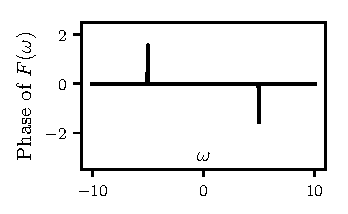
\includegraphics[width=0.325\textwidth]{phase_sin_signal}}%\label{fig:sin_signal_phase}
\caption{A continous fuction (a), and the real part (b), imaginary part (c), magnitude (d) and phase (e) of its Fourier transform.}\label{fig:sin_signal_fourier_comp}
\end{figure}

Figures demonstrate the result for a signal with $\omega_0=5$ and $A=2$. Figure  shows the continuous signal and  the real and imaginary parts and the magnitude and phase of its Fourier transform.  Figure  shows various windowed parts of the signal ($h(t)$) and the real and imaginary parts of their corresponding Fourier transforms.  Figure is the same as figure , but it shows the magnitude and phase of each Fourier transform. These Fourier transforms should be compared with their counterparts in figure  in order to appreciate the effect of both the size of the window and the locality of the window (Gaussian function). In all cases the main peaks of the Fourier transform's magnitude, which correspond to delta function impulses at $\omega=\pm 5$ in the continuous case, are preserved, but they become less sharp and the recovered value starts to move away from the real value as soon as the size of the window decreases. 

For the analysis of discrete signals it is possible to estimate the uncertainty principle. The easiest way is to consider signal segments and calculate the discrete Fourier transform (DFT) of each segment. This is the so-called Short Time Fourier Transform (STFT). If we consider an odd-sized window and associate the DFT that we calculate within it with the sample in the center of the window, we will be associating each sample of the signal with a ``small'' Fourier transform. In this context, how ``small'' the DTF is depends on the size of the window.



\begin{figure}
\centering
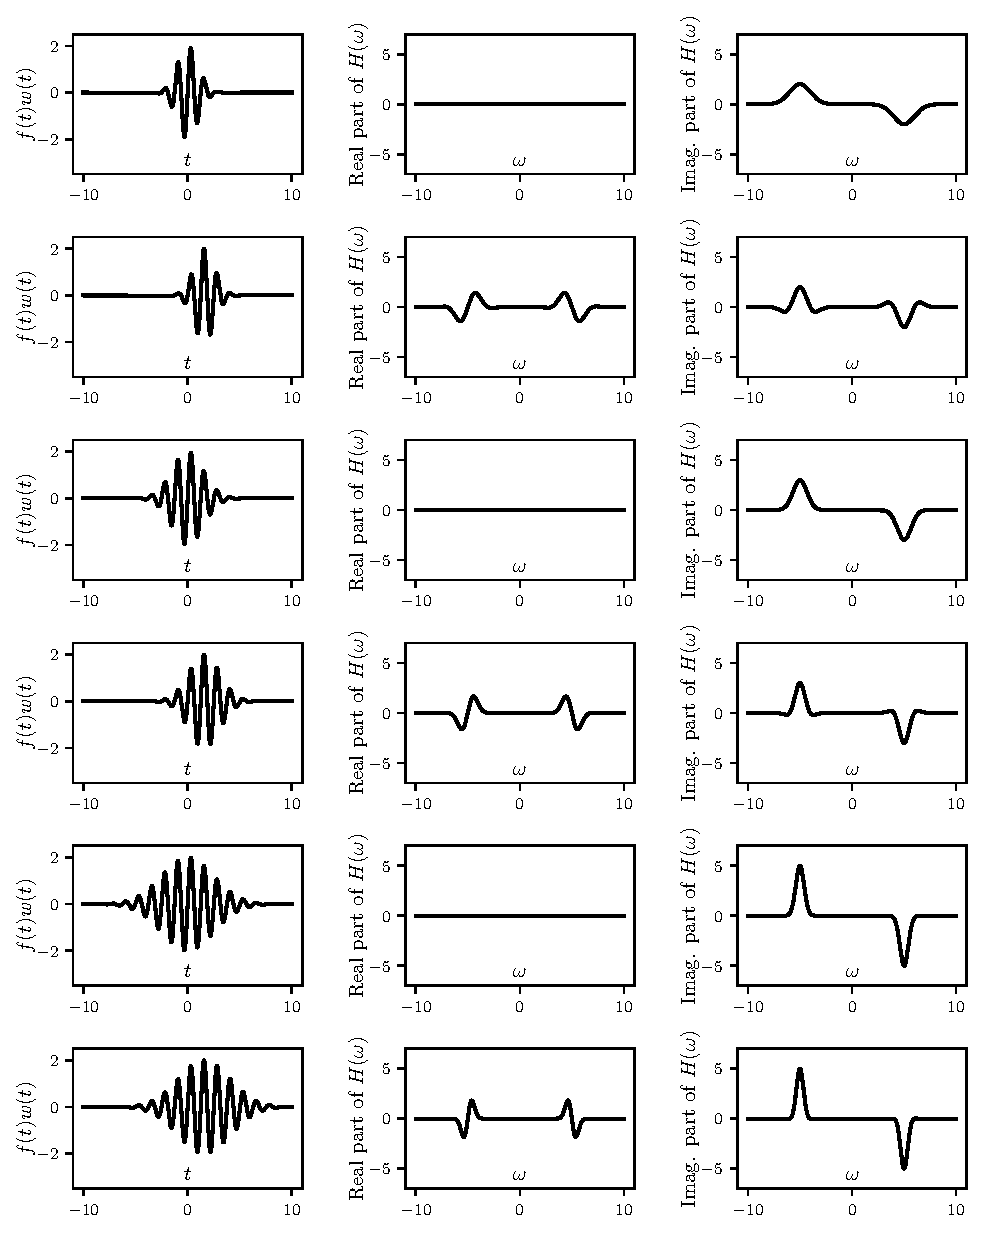
\includegraphics{sin_gauss_real_imag.pdf}
\caption{The effect of Gaussian window. Sinusoidal signal bounded by a Gaussian window (first column) and the real and imaginary part of its corresponding Fourier transform (second and third columns). From top to bottom: $[\sigma=1, t_0=0]$, $[\sigma=1, t_0=1.6]$, $[\sigma=1.5, t_0=0]$, $[\sigma=1.5, t_0=1.6]$, $[\sigma=2.5, t_0=0]$, $[\sigma=2.5, t_0=1.6]$.}\label{fig:gaussian_window_real_imag}
\end{figure}

\begin{figure}
\centering
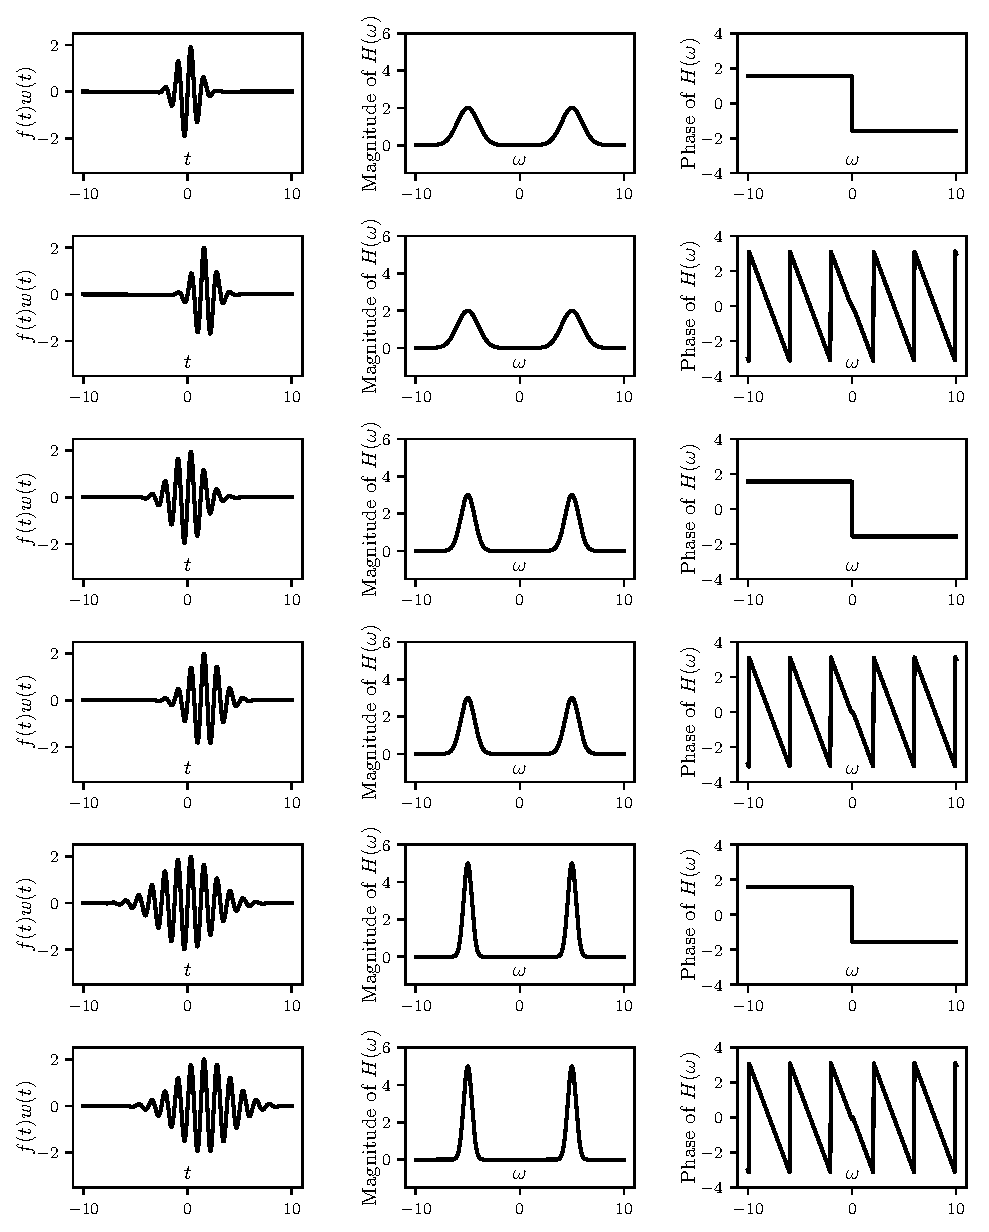
\includegraphics{sin_gauss_mag_phase.pdf}
\caption{The effect of Gaussian window. Sinusoidal signal bounded by a Gaussian window (first column) and the magnitude and phase of its corresponding Fourier transform (second and third columns). From top to bottom: $[\sigma=1, t_0=0]$, $[\sigma=1, t_0=1.6]$, $[\sigma=1.5, t_0=0]$, $[\sigma=1.5, t_0=1.6]$, $[\sigma=2.5, t_0=0]$, $[\sigma=2.5, t_0=1.6]$.}\label{fig:gaussian_window_mag_phase}
\end{figure}
